\documentclass[titlepage]{article}
\usepackage{graphicx}
\usepackage[a4paper,text={160mm,255mm},centering,headsep=5mm,footskip=10mm]{geometry}
\usepackage{nonfloat}
\parindent 0pt
\makeatletter
\newcommand\level[1]{%
   \ifcase#1\relax\expandafter\chapter\or
     \expandafter\section\or
     \expandafter\subsection\or
     \expandafter\subsubsection\else
     \def\next{\@level{#1}}\expandafter\next
   \fi}

\newcommand{\@level}[1]{%
\@startsection{level#1}
     {#1}
     {\z@}%
     {-3.25ex\@plus -1ex \@minus -.2ex}%
     {1.5ex \@plus .2ex}%
     {\normalfont\normalsize\bfseries}}

\newdimen\@leveldim
 \newdimen\@dotsdim
 {\normalfont\normalsize
  \sbox\z@{0}\global\@leveldim=\wd\z@
  \sbox\z@{.}\global\@dotsdim=\wd\z@
 }  
\newcounter{level4}[subsubsection]
 \@namedef{thelevel4}{\thesubsubsection.\arabic{level4}}
 \@namedef{level4mark}#1{}
 \def\l@section{\@dottedtocline{1}{0pt}{\dimexpr\@leveldim*4+\@dotsdim*1+6pt\relax}}
 \def\l@subsection{\@dottedtocline{2}{0pt}{\dimexpr\@leveldim*5+\@dotsdim*2+6pt\relax}}
 \def\l@subsubsection{\@dottedtocline{3}{0pt}{\dimexpr\@leveldim*6+\@dotsdim*3+6pt\relax}}
 \@namedef{l@level4}{\@dottedtocline{4}{0pt}{\dimexpr\@leveldim*7+\@dotsdim*4+6pt\relax}}

\count@=4
 \def\@ncp#1{\number\numexpr\count@+#1\relax}
 \loop\ifnum\count@<100
   \begingroup\edef\x{\endgroup
     \noexpand\newcounter{level\@ncp{1}}[level\number\count@]
     \noexpand\@namedef{thelevel\@ncp{1}}{%
       \noexpand\@nameuse{thelevel\@ncp{0}}.\noexpand\arabic{level\@ncp{0}}}
     \noexpand\@namedef{level\@ncp{1}mark}####1{}%
     \noexpand\@namedef{l@level\@ncp{1}}%
       {\noexpand\@dottedtocline{\@ncp{1}}{0pt}{\the\dimexpr\@leveldim*\@ncp{5}+\@dotsdim*\@ncp{0}\relax}}}%
   \x
   \advance\count@\@ne
 \repeat
 \makeatother
 \setcounter{secnumdepth}{100}
 \setcounter{tocdepth}{100}


\title{org.eclipse.etrice.examples.dynamicactors5 Model Documentation}
\date{\today}
\author{generated by eTrice}

\begin{document}
\pagestyle{plain}
\maketitle
\tableofcontents

\newpage
\listoffigures
\newpage
\section{Model Description}
\section{Logical System Description}
\level{2}{LS}
\level{3}{Instance Tree}
\begin{center}
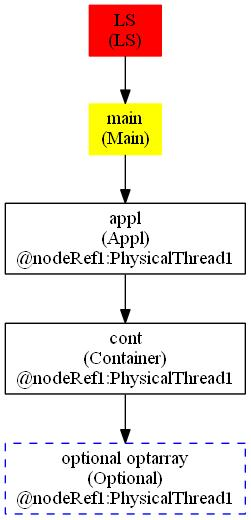
\includegraphics[scale=0.5]{C://Users//hrentz//Documents//protos//Entwicklung//Projekte//protos//eTrice//workspace//eTrice0.3.0//eTrice-dynact2-rt//org.eclipse.etrice.examples.dynamicactors5//doc-gen//images//LS_instanceTree.jpg}
\figcaption{LS Instance Tree}
\end{center}
\section{Subsystem Description}
\level{2}{Main}
\level{3}{Structure}
\begin{center}
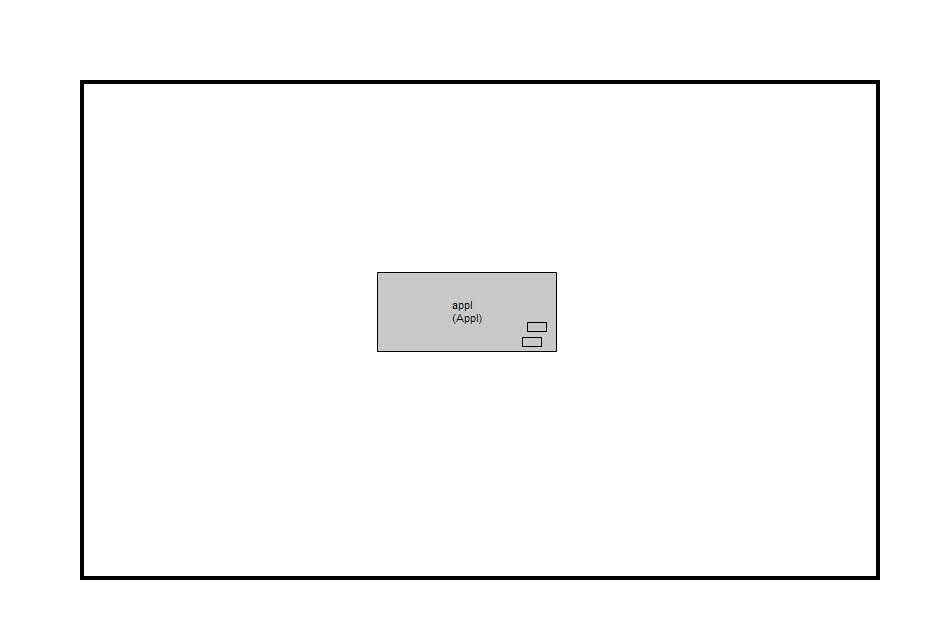
\includegraphics[scale=0.4]{C://Users//hrentz//Documents//protos//Entwicklung//Projekte//protos//eTrice//workspace//eTrice0.3.0//eTrice-dynact2-rt//org.eclipse.etrice.examples.dynamicactors5//doc-gen//images//Main_structure.jpg}
\figcaption{Main Structure}
\end{center}
\section{Protocol Class Description}
	\level{2} {PC}
	\level{3}{Incoming Messages}

	\begin{tabular}[ht]{|l|l|l|}
	\hline
	Message & Data & Description\\
	\hline
	sayHello &  & \\
	\hline
	\end{tabular}
	
	\level{3}{Outgoing Messages}
	\begin{tabular}[ht]{|l|l|l|}
	\hline
	Message & Data & Description\\
	\hline
	hello &  txt  & \\
	\hline
	\end{tabular}			
\section{Data Class Description}
\section{Actor Class Description}
\level{2}{Appl}
\level{3}{Structure}

\begin{center}
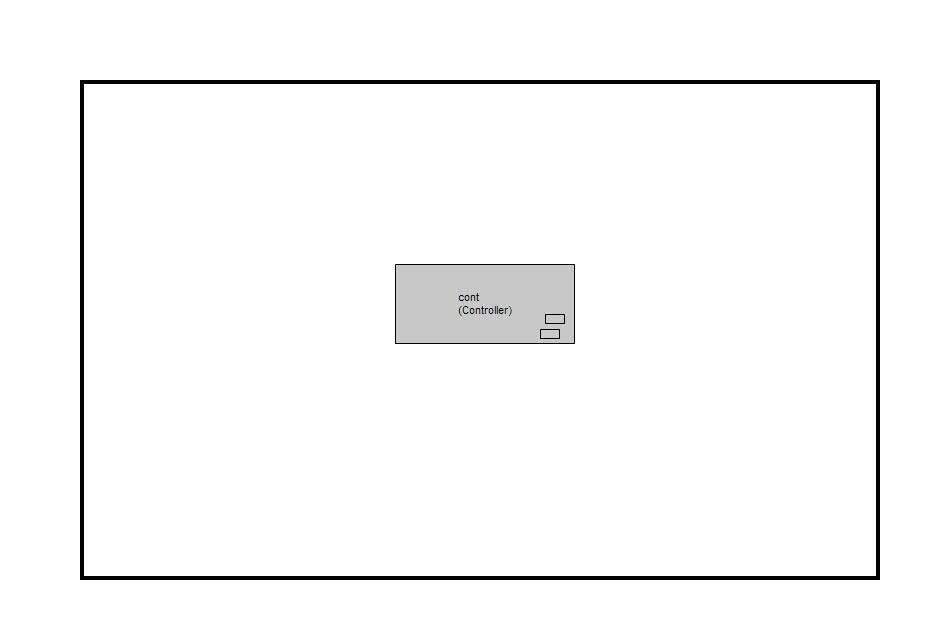
\includegraphics[scale=0.4]{C://Users//hrentz//Documents//protos//Entwicklung//Projekte//protos//eTrice//workspace//eTrice0.3.0//eTrice-dynact2-rt//org.eclipse.etrice.examples.dynamicactors5//doc-gen//images//Appl_structure.jpg}
\figcaption{Appl Structure}
\end{center}

\level{3}{Attributes}

\level{3}{Operations}
\level{2}{Container}
\level{3}{Structure}

\begin{center}
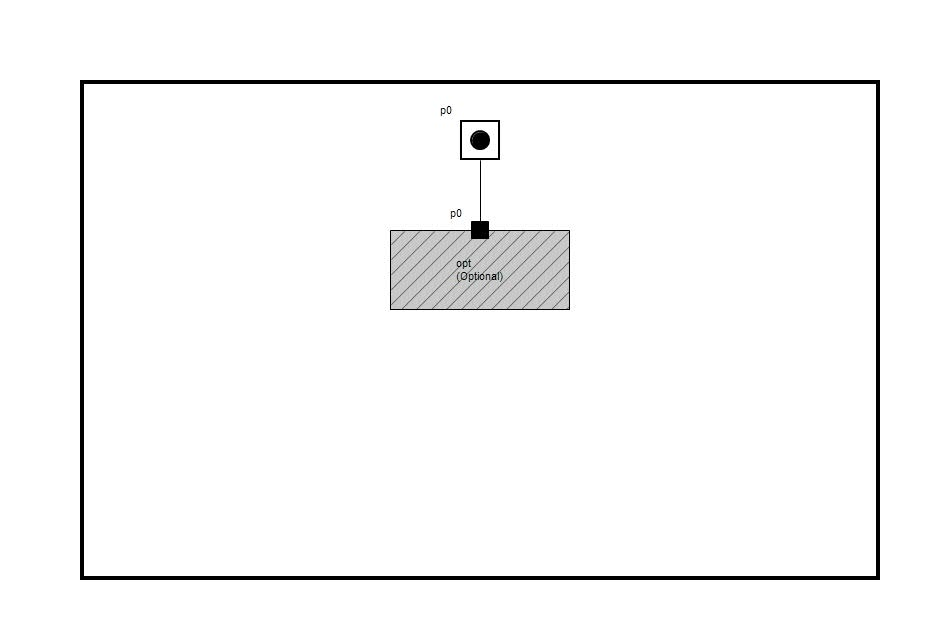
\includegraphics[scale=0.4]{C://Users//hrentz//Documents//protos//Entwicklung//Projekte//protos//eTrice//workspace//eTrice0.3.0//eTrice-dynact2-rt//org.eclipse.etrice.examples.dynamicactors5//doc-gen//images//Container_structure.jpg}
\figcaption{Container Structure}
\end{center}

\level{3}{Attributes}

\level{3}{Operations}
\begin{tabular}[ht]{|l|l|}
\hline		
	Name: & dumpTree\\
	\hline
	ReturnType: &  void\\
	\hline
	Arguments: & msg:string\\
	\hline
\end{tabular}
\newline\newline\newline
\level{3}{Statemachine}
\level{4}{Top Level}
\begin{center}
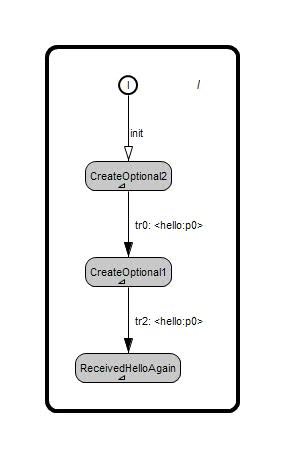
\includegraphics[scale=0.4]{C://Users//hrentz//Documents//protos//Entwicklung//Projekte//protos//eTrice//workspace//eTrice0.3.0//eTrice-dynact2-rt//org.eclipse.etrice.examples.dynamicactors5//doc-gen//images//Container_behavior.jpg}
\figcaption{Container Top State}
\end{center}

\begin{par}

\end{par}

\level{2}{Optional}
\level{3}{Structure}

\begin{center}
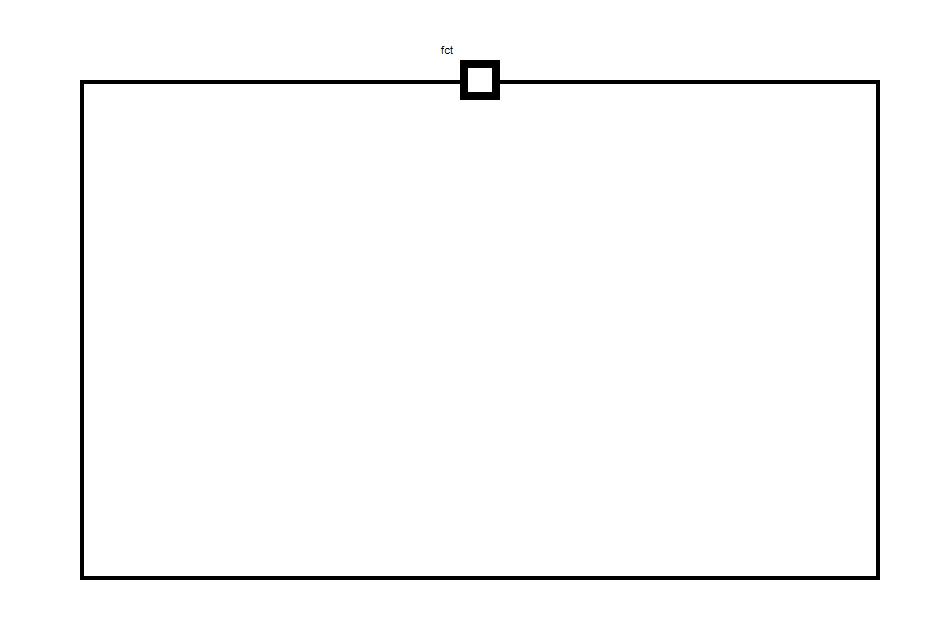
\includegraphics[scale=0.4]{C://Users//hrentz//Documents//protos//Entwicklung//Projekte//protos//eTrice//workspace//eTrice0.3.0//eTrice-dynact2-rt//org.eclipse.etrice.examples.dynamicactors5//doc-gen//images//Optional_structure.jpg}
\figcaption{Optional Structure}
\end{center}

\level{3}{Attributes}

\level{3}{Operations}
\level{3}{Statemachine}
\level{4}{Top Level}
\begin{center}
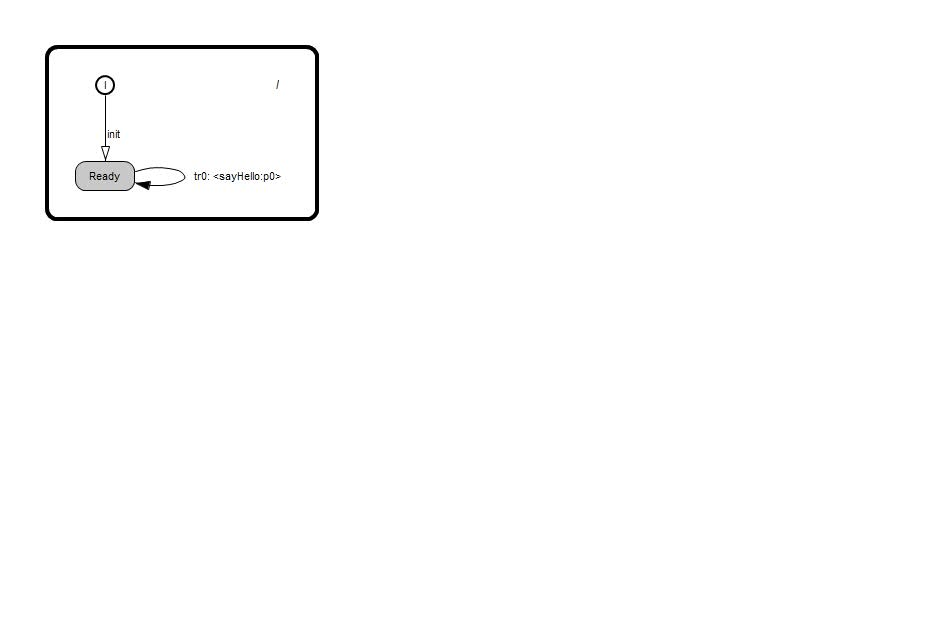
\includegraphics[scale=0.4]{C://Users//hrentz//Documents//protos//Entwicklung//Projekte//protos//eTrice//workspace//eTrice0.3.0//eTrice-dynact2-rt//org.eclipse.etrice.examples.dynamicactors5//doc-gen//images//Optional_behavior.jpg}
\figcaption{Optional Top State}
\end{center}

\begin{par}

\end{par}

\end{document}
